\section*{Výsledky měření}
Teplota v místnosti byla \SI{23.5(5)}{\degreeCelsius}.
Teplota destilované vody i lihu byla před smícháním stejná.

Drátek v rámečku jsme měřili posuvným měřítkem a měl délku $l = \SI{1.94(5)}{\cm}$.
Poloměr drátku byl $r = \SI{0.25(3)}{\milli\metre}$.
Rámeček měl hmotnost přibližně \SI{200}{\milli\g}.

Na váhy jsme pověsili přívažek o hmotnosti \SI{200}{\milli\g}.
Jelikož síly od sebe odečítáme, nemá přívažek na výsledek žádný vliv.

Torzními vahami jsme přímo měřili rozdíl hmotností na obou ramenech.
Ke změření síly je tedy nutný přepočet na tíhovou sílu $F = mg$, tedy
\begin{equation}
P_1 = m_1 \cdot g \qquad P_2= m_2 \cdot g \,,
\end{equation}
kde $m_1$, $m_2$ jsou váhami změřené rozdíly hmotností na ramenech, když je rámeček těsně pod vodou resp. právě se odtrhl od hladiny.
Tíhové zrychlení v Praze je \SI{9,814}{\m\per\s\squared} \cite{gravitace}, chybu zanedbáváme.

Nejdříve jsme změřili povrchové napětí čisté destilované vody a čistého lihu.
Poté jsme s pomocí pyknometru připravili roztok s \SI{50}{\percent} koncentrací lihu a tento roztok jsme dále ředili vodou vždy v poměru $1:1$.

V tabulce \ref{tab::namereny} jsou pro měřené koncentrace uvedeny hodnoty $m_1$, $m_2$, vypočtené síly $P_0$, přibližné hustoty $\varrho$ při dané koncentraci (hmotnostní koncentraci jsme odhadli objemovou koncentrací a hustotu určili z tabulek \cite{hustota}) a povrchové napětí~$\sigma$ podle \eqref{eq::lenard}.
U $m_1$ a $m_2$ uvádíme přímo číselný údaj na vahách, pro výpočet celkové hodnoty $P_1$ nebo $P_2$ by bylo nutné přičíst hmotnost přívažku.

Směrodatnou odchylku $\mu_m$\footnote{Symbol $\mu$ pro směrodatnou odchylku používáme, aby nedošlo k záměně za povrchové napětí $\sigma$.} určení rozdílu hmotností $(m_2-m_1)$ odhadujeme na \SI{5}{\milli \g}.
Z toho se odvíjí směrodatná odchylka síly $\mu_{P_0} = \SI{0.05}{\milli \newton}$.
Směrodatnou odchylku povrchového napětí počítáme jako
\begin{equation}
\mu_\sigma = \sigma \sqrt{ \left(  \frac{\mu_{P_0}}{P_0} \right)^2 +
\left(  \frac{\mu_{l}}{l} \right)^2   } \,.
\end{equation}

Chybu členu s $r$ ve vztahu \eqref{eq::lenard} zanedbáváme s ohledem na to, že je o řád menší než první zlomek.

Závislost povrchového napětí na koncentraci lihu v roztoku je zanesena do grafu \ref{grp::graf}.

\begin{tabulka}[htbp]
\centering
\begin{tabular}{cccccc}
koncentrace lihu & $m_1 (\si{\milli\g})$ & $m_2 (\si{\milli\g})$ & $P_0 (\si{\milli \newton})$ & $\varrho (\si{\kg\per\metre\cubed})$ & $\sigma (\num{e-3}\,\si{\newton\per\metre})$ \\ \hline 
\SI{0}{\percent} & \num{125} & \num{448} & \num{3.17} & \num{998} & \num{74(3)} \\
\SI{0.4}{\percent} & \num{118} & \num{430} & \num{3.06} & \num{997} & \num{71(3)} \\
\SI{0.8}{\percent} & \num{117} & \num{419} & \num{2.96} & \num{996} & \num{69(3)} \\
\SI{1.6}{\percent} & \num{113} & \num{404} & \num{2.86} & \num{995} & \num{66(3)} \\
\SI{3.1}{\percent} & \num{116} & \num{401} & \num{2.80} & \num{989} & \num{65(3)} \\
\SI{6.3}{\percent} & \num{111} & \num{370} & \num{2.54} & \num{987} & \num{58(3)} \\
\SI{12.5}{\percent} & \num{109} & \num{327} & \num{2.14} & \num{978} & \num{48(2)} \\
\SI{25}{\percent} & \num{106} & \num{277} & \num{1.68} & \num{962} & \num{37(2)} \\
\SI{50}{\percent} & \num{105} & \num{238} & \num{1.31} & \num{915} & \num{28(2)} \\
\SI{100}{\percent} & \num{106} & \num{225} & \num{1.17} & \num{789} & \num{25(2)} \\
\end{tabular}
\caption{Naměřené hodnoty povrchového napětí pro různé koncentrace lihu v roztoku}
\label{tab::namereny}
\end{tabulka}

\begin{graph}[htbp] 
\centering
% GNUPLOT: LaTeX picture with Postscript
\begingroup
  \makeatletter
  \providecommand\color[2][]{%
    \GenericError{(gnuplot) \space\space\space\@spaces}{%
      Package color not loaded in conjunction with
      terminal option `colourtext'%
    }{See the gnuplot documentation for explanation.%
    }{Either use 'blacktext' in gnuplot or load the package
      color.sty in LaTeX.}%
    \renewcommand\color[2][]{}%
  }%
  \providecommand\includegraphics[2][]{%
    \GenericError{(gnuplot) \space\space\space\@spaces}{%
      Package graphicx or graphics not loaded%
    }{See the gnuplot documentation for explanation.%
    }{The gnuplot epslatex terminal needs graphicx.sty or graphics.sty.}%
    \renewcommand\includegraphics[2][]{}%
  }%
  \providecommand\rotatebox[2]{#2}%
  \@ifundefined{ifGPcolor}{%
    \newif\ifGPcolor
    \GPcolorfalse
  }{}%
  \@ifundefined{ifGPblacktext}{%
    \newif\ifGPblacktext
    \GPblacktexttrue
  }{}%
  % define a \g@addto@macro without @ in the name:
  \let\gplgaddtomacro\g@addto@macro
  % define empty templates for all commands taking text:
  \gdef\gplbacktext{}%
  \gdef\gplfronttext{}%
  \makeatother
  \ifGPblacktext
    % no textcolor at all
    \def\colorrgb#1{}%
    \def\colorgray#1{}%
  \else
    % gray or color?
    \ifGPcolor
      \def\colorrgb#1{\color[rgb]{#1}}%
      \def\colorgray#1{\color[gray]{#1}}%
      \expandafter\def\csname LTw\endcsname{\color{white}}%
      \expandafter\def\csname LTb\endcsname{\color{black}}%
      \expandafter\def\csname LTa\endcsname{\color{black}}%
      \expandafter\def\csname LT0\endcsname{\color[rgb]{1,0,0}}%
      \expandafter\def\csname LT1\endcsname{\color[rgb]{0,1,0}}%
      \expandafter\def\csname LT2\endcsname{\color[rgb]{0,0,1}}%
      \expandafter\def\csname LT3\endcsname{\color[rgb]{1,0,1}}%
      \expandafter\def\csname LT4\endcsname{\color[rgb]{0,1,1}}%
      \expandafter\def\csname LT5\endcsname{\color[rgb]{1,1,0}}%
      \expandafter\def\csname LT6\endcsname{\color[rgb]{0,0,0}}%
      \expandafter\def\csname LT7\endcsname{\color[rgb]{1,0.3,0}}%
      \expandafter\def\csname LT8\endcsname{\color[rgb]{0.5,0.5,0.5}}%
    \else
      % gray
      \def\colorrgb#1{\color{black}}%
      \def\colorgray#1{\color[gray]{#1}}%
      \expandafter\def\csname LTw\endcsname{\color{white}}%
      \expandafter\def\csname LTb\endcsname{\color{black}}%
      \expandafter\def\csname LTa\endcsname{\color{black}}%
      \expandafter\def\csname LT0\endcsname{\color{black}}%
      \expandafter\def\csname LT1\endcsname{\color{black}}%
      \expandafter\def\csname LT2\endcsname{\color{black}}%
      \expandafter\def\csname LT3\endcsname{\color{black}}%
      \expandafter\def\csname LT4\endcsname{\color{black}}%
      \expandafter\def\csname LT5\endcsname{\color{black}}%
      \expandafter\def\csname LT6\endcsname{\color{black}}%
      \expandafter\def\csname LT7\endcsname{\color{black}}%
      \expandafter\def\csname LT8\endcsname{\color{black}}%
    \fi
  \fi
  \setlength{\unitlength}{0.0500bp}%
  \begin{picture}(10204.00,6802.00)%
    \gplgaddtomacro\gplbacktext{%
      \csname LTb\endcsname%
      \put(814,704){\makebox(0,0)[r]{\strut{} 20}}%
      \csname LTb\endcsname%
      \put(814,1537){\makebox(0,0)[r]{\strut{} 30}}%
      \csname LTb\endcsname%
      \put(814,2371){\makebox(0,0)[r]{\strut{} 40}}%
      \csname LTb\endcsname%
      \put(814,3204){\makebox(0,0)[r]{\strut{} 50}}%
      \csname LTb\endcsname%
      \put(814,4037){\makebox(0,0)[r]{\strut{} 60}}%
      \csname LTb\endcsname%
      \put(814,4870){\makebox(0,0)[r]{\strut{} 70}}%
      \csname LTb\endcsname%
      \put(814,5704){\makebox(0,0)[r]{\strut{} 80}}%
      \csname LTb\endcsname%
      \put(814,6537){\makebox(0,0)[r]{\strut{} 90}}%
      \csname LTb\endcsname%
      \put(946,484){\makebox(0,0){\strut{} 0}}%
      \csname LTb\endcsname%
      \put(2718,484){\makebox(0,0){\strut{} 20}}%
      \csname LTb\endcsname%
      \put(4490,484){\makebox(0,0){\strut{} 40}}%
      \csname LTb\endcsname%
      \put(6263,484){\makebox(0,0){\strut{} 60}}%
      \csname LTb\endcsname%
      \put(8035,484){\makebox(0,0){\strut{} 80}}%
      \csname LTb\endcsname%
      \put(9807,484){\makebox(0,0){\strut{} 100}}%
      \put(176,3620){\rotatebox{-270}{\makebox(0,0){\strut{}Povrchové napětí (\num{e-3}\,\si{\newton\per\metre})}}}%
      \put(5376,154){\makebox(0,0){\strut{}Koncentrace lihu (\si{\percent})}}%
    }%
    \gplgaddtomacro\gplfronttext{%
    }%
    \gplbacktext
    \put(0,0){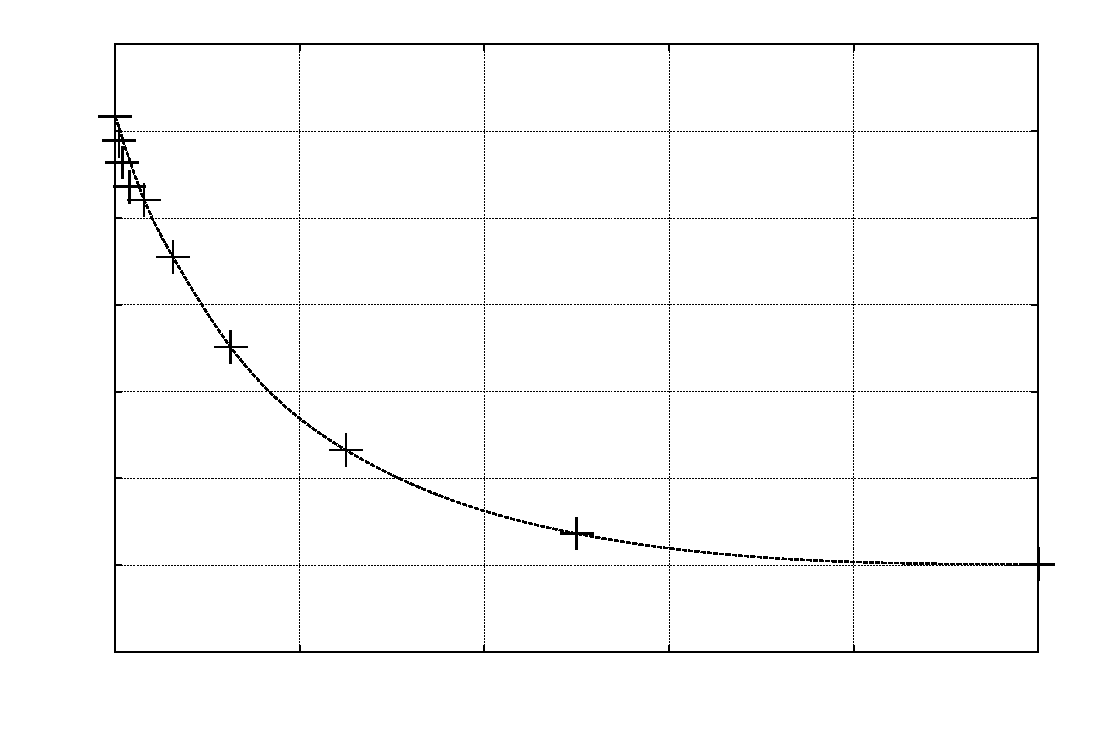
\includegraphics{graf}}%
    \gplfronttext
  \end{picture}%
\endgroup

\caption{Závislost povrchového napětí na koncentraci lihu v roztoku}
\label{grp::graf}
\end{graph}